
% Default to the notebook output style

    


% Inherit from the specified cell style.




    
\documentclass[11pt]{article}

    
    
    \usepackage[T1]{fontenc}
    % Nicer default font than Computer Modern for most use cases
    \usepackage{palatino}

    % Basic figure setup, for now with no caption control since it's done
    % automatically by Pandoc (which extracts ![](path) syntax from Markdown).
    \usepackage{graphicx}
    % We will generate all images so they have a width \maxwidth. This means
    % that they will get their normal width if they fit onto the page, but
    % are scaled down if they would overflow the margins.
    \makeatletter
    \def\maxwidth{\ifdim\Gin@nat@width>\linewidth\linewidth
    \else\Gin@nat@width\fi}
    \makeatother
    \let\Oldincludegraphics\includegraphics
    % Set max figure width to be 80% of text width, for now hardcoded.
    \renewcommand{\includegraphics}[1]{\Oldincludegraphics[width=.8\maxwidth]{#1}}
    % Ensure that by default, figures have no caption (until we provide a
    % proper Figure object with a Caption API and a way to capture that
    % in the conversion process - todo).
    \usepackage{caption}
    \DeclareCaptionLabelFormat{nolabel}{}
    \captionsetup{labelformat=nolabel}

    \usepackage{adjustbox} % Used to constrain images to a maximum size 
    \usepackage{xcolor} % Allow colors to be defined
    \usepackage{enumerate} % Needed for markdown enumerations to work
    \usepackage{geometry} % Used to adjust the document margins
    \usepackage{amsmath} % Equations
    \usepackage{amssymb} % Equations
    \usepackage{textcomp} % defines textquotesingle
    % Hack from http://tex.stackexchange.com/a/47451/13684:
    \AtBeginDocument{%
        \def\PYZsq{\textquotesingle}% Upright quotes in Pygmentized code
    }
    \usepackage{upquote} % Upright quotes for verbatim code
    \usepackage{eurosym} % defines \euro
    \usepackage[mathletters]{ucs} % Extended unicode (utf-8) support
    \usepackage[utf8x]{inputenc} % Allow utf-8 characters in the tex document
    \usepackage{fancyvrb} % verbatim replacement that allows latex
    \usepackage{grffile} % extends the file name processing of package graphics 
                         % to support a larger range 
    % The hyperref package gives us a pdf with properly built
    % internal navigation ('pdf bookmarks' for the table of contents,
    % internal cross-reference links, web links for URLs, etc.)
    \usepackage{hyperref}
    \usepackage{longtable} % longtable support required by pandoc >1.10
    \usepackage{booktabs}  % table support for pandoc > 1.12.2
    \usepackage[normalem]{ulem} % ulem is needed to support strikethroughs (\sout)
                                % normalem makes italics be italics, not underlines
    

    
    
    % Colors for the hyperref package
    \definecolor{urlcolor}{rgb}{0,.145,.698}
    \definecolor{linkcolor}{rgb}{.71,0.21,0.01}
    \definecolor{citecolor}{rgb}{.12,.54,.11}

    % ANSI colors
    \definecolor{ansi-black}{HTML}{3E424D}
    \definecolor{ansi-black-intense}{HTML}{282C36}
    \definecolor{ansi-red}{HTML}{E75C58}
    \definecolor{ansi-red-intense}{HTML}{B22B31}
    \definecolor{ansi-green}{HTML}{00A250}
    \definecolor{ansi-green-intense}{HTML}{007427}
    \definecolor{ansi-yellow}{HTML}{DDB62B}
    \definecolor{ansi-yellow-intense}{HTML}{B27D12}
    \definecolor{ansi-blue}{HTML}{208FFB}
    \definecolor{ansi-blue-intense}{HTML}{0065CA}
    \definecolor{ansi-magenta}{HTML}{D160C4}
    \definecolor{ansi-magenta-intense}{HTML}{A03196}
    \definecolor{ansi-cyan}{HTML}{60C6C8}
    \definecolor{ansi-cyan-intense}{HTML}{258F8F}
    \definecolor{ansi-white}{HTML}{C5C1B4}
    \definecolor{ansi-white-intense}{HTML}{A1A6B2}

    % commands and environments needed by pandoc snippets
    % extracted from the output of `pandoc -s`
    \providecommand{\tightlist}{%
      \setlength{\itemsep}{0pt}\setlength{\parskip}{0pt}}
    \DefineVerbatimEnvironment{Highlighting}{Verbatim}{commandchars=\\\{\}}
    % Add ',fontsize=\small' for more characters per line
    \newenvironment{Shaded}{}{}
    \newcommand{\KeywordTok}[1]{\textcolor[rgb]{0.00,0.44,0.13}{\textbf{{#1}}}}
    \newcommand{\DataTypeTok}[1]{\textcolor[rgb]{0.56,0.13,0.00}{{#1}}}
    \newcommand{\DecValTok}[1]{\textcolor[rgb]{0.25,0.63,0.44}{{#1}}}
    \newcommand{\BaseNTok}[1]{\textcolor[rgb]{0.25,0.63,0.44}{{#1}}}
    \newcommand{\FloatTok}[1]{\textcolor[rgb]{0.25,0.63,0.44}{{#1}}}
    \newcommand{\CharTok}[1]{\textcolor[rgb]{0.25,0.44,0.63}{{#1}}}
    \newcommand{\StringTok}[1]{\textcolor[rgb]{0.25,0.44,0.63}{{#1}}}
    \newcommand{\CommentTok}[1]{\textcolor[rgb]{0.38,0.63,0.69}{\textit{{#1}}}}
    \newcommand{\OtherTok}[1]{\textcolor[rgb]{0.00,0.44,0.13}{{#1}}}
    \newcommand{\AlertTok}[1]{\textcolor[rgb]{1.00,0.00,0.00}{\textbf{{#1}}}}
    \newcommand{\FunctionTok}[1]{\textcolor[rgb]{0.02,0.16,0.49}{{#1}}}
    \newcommand{\RegionMarkerTok}[1]{{#1}}
    \newcommand{\ErrorTok}[1]{\textcolor[rgb]{1.00,0.00,0.00}{\textbf{{#1}}}}
    \newcommand{\NormalTok}[1]{{#1}}
    
    % Additional commands for more recent versions of Pandoc
    \newcommand{\ConstantTok}[1]{\textcolor[rgb]{0.53,0.00,0.00}{{#1}}}
    \newcommand{\SpecialCharTok}[1]{\textcolor[rgb]{0.25,0.44,0.63}{{#1}}}
    \newcommand{\VerbatimStringTok}[1]{\textcolor[rgb]{0.25,0.44,0.63}{{#1}}}
    \newcommand{\SpecialStringTok}[1]{\textcolor[rgb]{0.73,0.40,0.53}{{#1}}}
    \newcommand{\ImportTok}[1]{{#1}}
    \newcommand{\DocumentationTok}[1]{\textcolor[rgb]{0.73,0.13,0.13}{\textit{{#1}}}}
    \newcommand{\AnnotationTok}[1]{\textcolor[rgb]{0.38,0.63,0.69}{\textbf{\textit{{#1}}}}}
    \newcommand{\CommentVarTok}[1]{\textcolor[rgb]{0.38,0.63,0.69}{\textbf{\textit{{#1}}}}}
    \newcommand{\VariableTok}[1]{\textcolor[rgb]{0.10,0.09,0.49}{{#1}}}
    \newcommand{\ControlFlowTok}[1]{\textcolor[rgb]{0.00,0.44,0.13}{\textbf{{#1}}}}
    \newcommand{\OperatorTok}[1]{\textcolor[rgb]{0.40,0.40,0.40}{{#1}}}
    \newcommand{\BuiltInTok}[1]{{#1}}
    \newcommand{\ExtensionTok}[1]{{#1}}
    \newcommand{\PreprocessorTok}[1]{\textcolor[rgb]{0.74,0.48,0.00}{{#1}}}
    \newcommand{\AttributeTok}[1]{\textcolor[rgb]{0.49,0.56,0.16}{{#1}}}
    \newcommand{\InformationTok}[1]{\textcolor[rgb]{0.38,0.63,0.69}{\textbf{\textit{{#1}}}}}
    \newcommand{\WarningTok}[1]{\textcolor[rgb]{0.38,0.63,0.69}{\textbf{\textit{{#1}}}}}
    
    
    % Define a nice break command that doesn't care if a line doesn't already
    % exist.
    \def\br{\hspace*{\fill} \\* }
    % Math Jax compatability definitions
    \def\gt{>}
    \def\lt{<}
    % Document parameters
    \title{GSoC 2017 Application Ayush Pandey- Optimization and Bayesian Techniques for the parameter estimation of Differential Equations}
    
    
    

    % Pygments definitions
    
\makeatletter
\def\PY@reset{\let\PY@it=\relax \let\PY@bf=\relax%
    \let\PY@ul=\relax \let\PY@tc=\relax%
    \let\PY@bc=\relax \let\PY@ff=\relax}
\def\PY@tok#1{\csname PY@tok@#1\endcsname}
\def\PY@toks#1+{\ifx\relax#1\empty\else%
    \PY@tok{#1}\expandafter\PY@toks\fi}
\def\PY@do#1{\PY@bc{\PY@tc{\PY@ul{%
    \PY@it{\PY@bf{\PY@ff{#1}}}}}}}
\def\PY#1#2{\PY@reset\PY@toks#1+\relax+\PY@do{#2}}

\expandafter\def\csname PY@tok@m\endcsname{\def\PY@tc##1{\textcolor[rgb]{0.40,0.40,0.40}{##1}}}
\expandafter\def\csname PY@tok@nf\endcsname{\def\PY@tc##1{\textcolor[rgb]{0.00,0.00,1.00}{##1}}}
\expandafter\def\csname PY@tok@sc\endcsname{\def\PY@tc##1{\textcolor[rgb]{0.73,0.13,0.13}{##1}}}
\expandafter\def\csname PY@tok@c1\endcsname{\let\PY@it=\textit\def\PY@tc##1{\textcolor[rgb]{0.25,0.50,0.50}{##1}}}
\expandafter\def\csname PY@tok@err\endcsname{\def\PY@bc##1{\setlength{\fboxsep}{0pt}\fcolorbox[rgb]{1.00,0.00,0.00}{1,1,1}{\strut ##1}}}
\expandafter\def\csname PY@tok@gu\endcsname{\let\PY@bf=\textbf\def\PY@tc##1{\textcolor[rgb]{0.50,0.00,0.50}{##1}}}
\expandafter\def\csname PY@tok@sb\endcsname{\def\PY@tc##1{\textcolor[rgb]{0.73,0.13,0.13}{##1}}}
\expandafter\def\csname PY@tok@gh\endcsname{\let\PY@bf=\textbf\def\PY@tc##1{\textcolor[rgb]{0.00,0.00,0.50}{##1}}}
\expandafter\def\csname PY@tok@na\endcsname{\def\PY@tc##1{\textcolor[rgb]{0.49,0.56,0.16}{##1}}}
\expandafter\def\csname PY@tok@go\endcsname{\def\PY@tc##1{\textcolor[rgb]{0.53,0.53,0.53}{##1}}}
\expandafter\def\csname PY@tok@kp\endcsname{\def\PY@tc##1{\textcolor[rgb]{0.00,0.50,0.00}{##1}}}
\expandafter\def\csname PY@tok@ow\endcsname{\let\PY@bf=\textbf\def\PY@tc##1{\textcolor[rgb]{0.67,0.13,1.00}{##1}}}
\expandafter\def\csname PY@tok@s1\endcsname{\def\PY@tc##1{\textcolor[rgb]{0.73,0.13,0.13}{##1}}}
\expandafter\def\csname PY@tok@nv\endcsname{\def\PY@tc##1{\textcolor[rgb]{0.10,0.09,0.49}{##1}}}
\expandafter\def\csname PY@tok@mo\endcsname{\def\PY@tc##1{\textcolor[rgb]{0.40,0.40,0.40}{##1}}}
\expandafter\def\csname PY@tok@cm\endcsname{\let\PY@it=\textit\def\PY@tc##1{\textcolor[rgb]{0.25,0.50,0.50}{##1}}}
\expandafter\def\csname PY@tok@nt\endcsname{\let\PY@bf=\textbf\def\PY@tc##1{\textcolor[rgb]{0.00,0.50,0.00}{##1}}}
\expandafter\def\csname PY@tok@sh\endcsname{\def\PY@tc##1{\textcolor[rgb]{0.73,0.13,0.13}{##1}}}
\expandafter\def\csname PY@tok@se\endcsname{\let\PY@bf=\textbf\def\PY@tc##1{\textcolor[rgb]{0.73,0.40,0.13}{##1}}}
\expandafter\def\csname PY@tok@si\endcsname{\let\PY@bf=\textbf\def\PY@tc##1{\textcolor[rgb]{0.73,0.40,0.53}{##1}}}
\expandafter\def\csname PY@tok@kd\endcsname{\let\PY@bf=\textbf\def\PY@tc##1{\textcolor[rgb]{0.00,0.50,0.00}{##1}}}
\expandafter\def\csname PY@tok@gd\endcsname{\def\PY@tc##1{\textcolor[rgb]{0.63,0.00,0.00}{##1}}}
\expandafter\def\csname PY@tok@s\endcsname{\def\PY@tc##1{\textcolor[rgb]{0.73,0.13,0.13}{##1}}}
\expandafter\def\csname PY@tok@c\endcsname{\let\PY@it=\textit\def\PY@tc##1{\textcolor[rgb]{0.25,0.50,0.50}{##1}}}
\expandafter\def\csname PY@tok@ch\endcsname{\let\PY@it=\textit\def\PY@tc##1{\textcolor[rgb]{0.25,0.50,0.50}{##1}}}
\expandafter\def\csname PY@tok@sx\endcsname{\def\PY@tc##1{\textcolor[rgb]{0.00,0.50,0.00}{##1}}}
\expandafter\def\csname PY@tok@kn\endcsname{\let\PY@bf=\textbf\def\PY@tc##1{\textcolor[rgb]{0.00,0.50,0.00}{##1}}}
\expandafter\def\csname PY@tok@ss\endcsname{\def\PY@tc##1{\textcolor[rgb]{0.10,0.09,0.49}{##1}}}
\expandafter\def\csname PY@tok@cs\endcsname{\let\PY@it=\textit\def\PY@tc##1{\textcolor[rgb]{0.25,0.50,0.50}{##1}}}
\expandafter\def\csname PY@tok@gs\endcsname{\let\PY@bf=\textbf}
\expandafter\def\csname PY@tok@nc\endcsname{\let\PY@bf=\textbf\def\PY@tc##1{\textcolor[rgb]{0.00,0.00,1.00}{##1}}}
\expandafter\def\csname PY@tok@s2\endcsname{\def\PY@tc##1{\textcolor[rgb]{0.73,0.13,0.13}{##1}}}
\expandafter\def\csname PY@tok@gp\endcsname{\let\PY@bf=\textbf\def\PY@tc##1{\textcolor[rgb]{0.00,0.00,0.50}{##1}}}
\expandafter\def\csname PY@tok@vc\endcsname{\def\PY@tc##1{\textcolor[rgb]{0.10,0.09,0.49}{##1}}}
\expandafter\def\csname PY@tok@o\endcsname{\def\PY@tc##1{\textcolor[rgb]{0.40,0.40,0.40}{##1}}}
\expandafter\def\csname PY@tok@nb\endcsname{\def\PY@tc##1{\textcolor[rgb]{0.00,0.50,0.00}{##1}}}
\expandafter\def\csname PY@tok@gr\endcsname{\def\PY@tc##1{\textcolor[rgb]{1.00,0.00,0.00}{##1}}}
\expandafter\def\csname PY@tok@kt\endcsname{\def\PY@tc##1{\textcolor[rgb]{0.69,0.00,0.25}{##1}}}
\expandafter\def\csname PY@tok@mi\endcsname{\def\PY@tc##1{\textcolor[rgb]{0.40,0.40,0.40}{##1}}}
\expandafter\def\csname PY@tok@w\endcsname{\def\PY@tc##1{\textcolor[rgb]{0.73,0.73,0.73}{##1}}}
\expandafter\def\csname PY@tok@mh\endcsname{\def\PY@tc##1{\textcolor[rgb]{0.40,0.40,0.40}{##1}}}
\expandafter\def\csname PY@tok@vg\endcsname{\def\PY@tc##1{\textcolor[rgb]{0.10,0.09,0.49}{##1}}}
\expandafter\def\csname PY@tok@gt\endcsname{\def\PY@tc##1{\textcolor[rgb]{0.00,0.27,0.87}{##1}}}
\expandafter\def\csname PY@tok@nn\endcsname{\let\PY@bf=\textbf\def\PY@tc##1{\textcolor[rgb]{0.00,0.00,1.00}{##1}}}
\expandafter\def\csname PY@tok@il\endcsname{\def\PY@tc##1{\textcolor[rgb]{0.40,0.40,0.40}{##1}}}
\expandafter\def\csname PY@tok@gi\endcsname{\def\PY@tc##1{\textcolor[rgb]{0.00,0.63,0.00}{##1}}}
\expandafter\def\csname PY@tok@nl\endcsname{\def\PY@tc##1{\textcolor[rgb]{0.63,0.63,0.00}{##1}}}
\expandafter\def\csname PY@tok@sr\endcsname{\def\PY@tc##1{\textcolor[rgb]{0.73,0.40,0.53}{##1}}}
\expandafter\def\csname PY@tok@ge\endcsname{\let\PY@it=\textit}
\expandafter\def\csname PY@tok@kr\endcsname{\let\PY@bf=\textbf\def\PY@tc##1{\textcolor[rgb]{0.00,0.50,0.00}{##1}}}
\expandafter\def\csname PY@tok@cp\endcsname{\def\PY@tc##1{\textcolor[rgb]{0.74,0.48,0.00}{##1}}}
\expandafter\def\csname PY@tok@mb\endcsname{\def\PY@tc##1{\textcolor[rgb]{0.40,0.40,0.40}{##1}}}
\expandafter\def\csname PY@tok@ne\endcsname{\let\PY@bf=\textbf\def\PY@tc##1{\textcolor[rgb]{0.82,0.25,0.23}{##1}}}
\expandafter\def\csname PY@tok@kc\endcsname{\let\PY@bf=\textbf\def\PY@tc##1{\textcolor[rgb]{0.00,0.50,0.00}{##1}}}
\expandafter\def\csname PY@tok@cpf\endcsname{\let\PY@it=\textit\def\PY@tc##1{\textcolor[rgb]{0.25,0.50,0.50}{##1}}}
\expandafter\def\csname PY@tok@mf\endcsname{\def\PY@tc##1{\textcolor[rgb]{0.40,0.40,0.40}{##1}}}
\expandafter\def\csname PY@tok@sd\endcsname{\let\PY@it=\textit\def\PY@tc##1{\textcolor[rgb]{0.73,0.13,0.13}{##1}}}
\expandafter\def\csname PY@tok@bp\endcsname{\def\PY@tc##1{\textcolor[rgb]{0.00,0.50,0.00}{##1}}}
\expandafter\def\csname PY@tok@k\endcsname{\let\PY@bf=\textbf\def\PY@tc##1{\textcolor[rgb]{0.00,0.50,0.00}{##1}}}
\expandafter\def\csname PY@tok@vi\endcsname{\def\PY@tc##1{\textcolor[rgb]{0.10,0.09,0.49}{##1}}}
\expandafter\def\csname PY@tok@ni\endcsname{\let\PY@bf=\textbf\def\PY@tc##1{\textcolor[rgb]{0.60,0.60,0.60}{##1}}}
\expandafter\def\csname PY@tok@nd\endcsname{\def\PY@tc##1{\textcolor[rgb]{0.67,0.13,1.00}{##1}}}
\expandafter\def\csname PY@tok@no\endcsname{\def\PY@tc##1{\textcolor[rgb]{0.53,0.00,0.00}{##1}}}

\def\PYZbs{\char`\\}
\def\PYZus{\char`\_}
\def\PYZob{\char`\{}
\def\PYZcb{\char`\}}
\def\PYZca{\char`\^}
\def\PYZam{\char`\&}
\def\PYZlt{\char`\<}
\def\PYZgt{\char`\>}
\def\PYZsh{\char`\#}
\def\PYZpc{\char`\%}
\def\PYZdl{\char`\$}
\def\PYZhy{\char`\-}
\def\PYZsq{\char`\'}
\def\PYZdq{\char`\"}
\def\PYZti{\char`\~}
% for compatibility with earlier versions
\def\PYZat{@}
\def\PYZlb{[}
\def\PYZrb{]}
\makeatother


    % Exact colors from NB
    \definecolor{incolor}{rgb}{0.0, 0.0, 0.5}
    \definecolor{outcolor}{rgb}{0.545, 0.0, 0.0}



    
    % Prevent overflowing lines due to hard-to-break entities
    \sloppy 
    % Setup hyperref package
    \hypersetup{
      breaklinks=true,  % so long urls are correctly broken across lines
      colorlinks=true,
      urlcolor=urlcolor,
      linkcolor=linkcolor,
      citecolor=citecolor,
      }
    % Slightly bigger margins than the latex defaults
    
    \geometry{verbose,tmargin=1in,bmargin=1in,lmargin=1in,rmargin=1in}
    
    

    \begin{document}
    
    
    \maketitle
    
    

    
    \section{Contact}\label{contact}

\textbf{Name} : Ayush Pandey

\textbf{University} : \href{http://iitkgp.ac.in}{Indian Institute of
Technology (IIT), Kharagpur}

\textbf{Email} : ayushpandey.iitkgp@gmail.com

\textbf{IRC Handle} : KrishnaKanhaiya at freenode.net

\textbf{Github Username} :
\href{https://github.com/Ayush-iitkgp}{Ayush-iitkgp}

\textbf{Mentor} : \href{https://github.com/ChrisRackauckas}{Christopher
Rackauckas}

    \section{The Project}\label{the-project}

\subsection{The Problem and
Motivations}\label{the-problem-and-motivations}

The aim of the project is to add different optimization and bayesian
techniques to estimate the parameters of the differential equation in
DiffEqParamEstim.jl package and do a comprehensive study of the pros and
cons of the different algorithms to add it to the documentation.

Differential equation models are widely used in many scientific fields
that include engineering, physics, and biomedical sciences. The
so-called ``forward problem'' that is the problem of solving
differential equations for given parameter values in the differential
equation models has been extensively studied by mathematicians,
physicists, engineers, and scientists.

However, the \textbf{inverse problem}, the problem of parameter
estimation based on the measurements of output variables, has not been
well explored using modern optimization and statistical methods.
Parameter estimation aims to find the unknown parameters of the model
which give the best fit to a set of experimental data. In this way,
parameters which cannot be measured directly will be determined in order
to ensure the best fit of the model with the experimental results. This
will be done by globally minimizing an objective function which measures
the quality of the fit. This inverse problem usually considers a cost
function to be optimized (such as maximum likelihood). This problem has
applications in systems biology, HIV-AIDS study, and drug dosage
estimation.

    \section{The Plan}\label{the-plan}

I propose to implement different algorithms for estimation of the
parameters of the differential equations such as:

\begin{enumerate}
\def\labelenumi{\arabic{enumi}.}
\tightlist
\item
  Implement support for more Kernels for two-stage method
\item
  Implement support for different distance measures such as
  (log-)likelihood and expectation maximization algorithm
\item
  Implement regularization techniques such as Tikhonov regularization,
  LASSO regularization and integrate with PenaltyFunctions.jl
\item
  Provide support for deterministic and heuristic algorithms for global
  optimum such as BlackBoxOptim, genetic algorithm
\item
  Implement Generalized Profiling Approach using Model Relaxation method
  for parameter estimation
\item
  Bayesian techniques for parameter estimation using Stan.jl
\end{enumerate}

\textbf{Stretch Goals}

\begin{enumerate}
\def\labelenumi{\arabic{enumi}.}
\tightlist
\item
  Implementing support for parameter estimation for stochastic
  differential equations
\item
  Writing native Julia bayesian computational engine using Mamba.jl and
  Klara.jl
\end{enumerate}

I also aim to do a detailed study of the methods and write a proper
documentation on where to use the algorithms, precautions to take while
using them and the pros and cons of the above methods.

\subsection{Mathematical Formulation}\label{mathematical-formulation}

First of all, we need to understand the mathematical formulation of the
inverse parameter estimation problem before we get into the
implementation details.

\subsubsection{General Form of Parameter Estimation
Problem}\label{general-form-of-parameter-estimation-problem}

\begin{figure}[htbp]
\centering
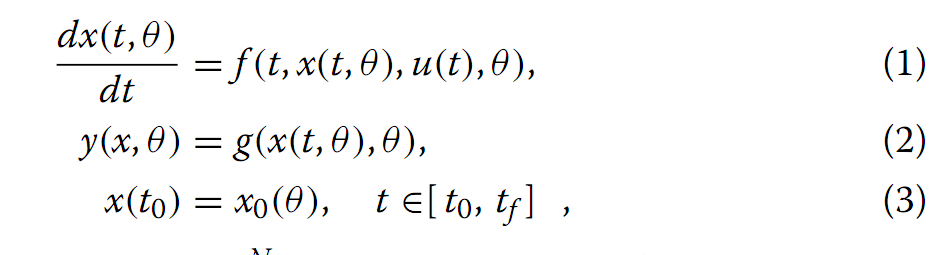
\includegraphics{images/General_Parameter_Estimation_Form.png}
\caption{}
\end{figure}

where \(x \in \mathbf{R}^{n}\) is the observed state vector,
\(\theta \in {R}^{m}\) is the vector of unknown parameters, f(.) is a
known linear or non-linear function vector. In general, we may not
observe x directly but we can observe a function of x, here g(.) is the
observation functions that maps the state variable to a vector of
observable quantities \(y \in {R}^{n}\), these are the signals that can
be measured in the experiments.

\subsubsection{Maximum likelihood and cost
function}\label{maximum-likelihood-and-cost-function}

Maximum likelihood and cost function Assuming that the transformed
measurements y are contaminated by additive normally distributed
uncorrelated random measurement errors i.e. \(y_{ijk}\) =
\(y_{ijk}(x(t_{i}), θ) + e_{ijk}\) where \(e_{ijk}\) ∼ N(0,
\(σ^{2}_{ijk})\) is the random error with standard deviation \(σ_{ijk}\)
and \(y_{ijk}\) is the measured value, the estimation of the model
parameters is formulated as the maximization of the likelihood of the
data:

\begin{figure}[htbp]
\centering
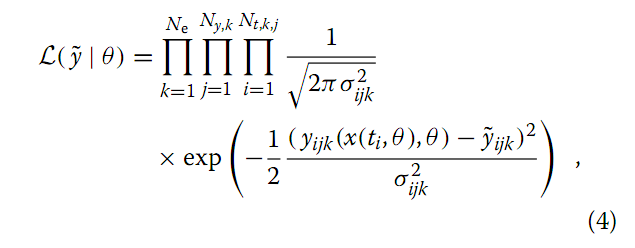
\includegraphics{images/Maximum_Likelihood.png}
\caption{}
\end{figure}

where \(N_{e}\) is the number of experiments, \(N_{y,k}\) is the number
of observed compounds in the kth experiment, and \(N_{t,k,j}\) is the
number of measurement time points of the jth observed quantity in the
kth experiment.

From the theory of maximum likelihood, \textbf{the objective is to
maximize the likelihood function} and estimate the parameters for which
the likelihood function is maximized.

Since the likelihood function consists of product terms, we take the log
of the likelihood function and negate it to ease our calculation, thus
we get log-likelihood function as follows:

\begin{figure}[htbp]
\centering
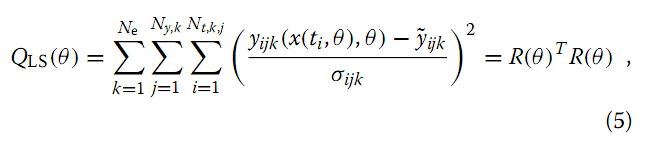
\includegraphics{images/Maximum_log_Likelihood.png}
\caption{}
\end{figure}

\textbf{Note} - The maximization of the likelihood function (4) is
equivalent to the minimization of the weighted least squares cost
function (5).

where the residual vector R(·) : \(R^{N_{θ}}\) → \(R^{N_{D}}\) is
constructed from the squared terms by arranging them to a vector. With
this, the model calibration problem can be stated as the well-known
nonlinear least-squares (NLS) optimization problem:

\begin{figure}[htbp]
\centering
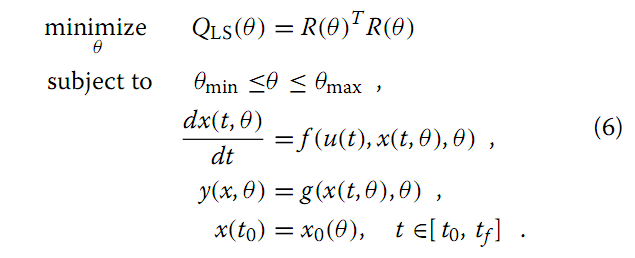
\includegraphics{images/NLS.png}
\caption{}
\end{figure}

A \(\theta\) vector that solves this optimization problem is called the
maximum-likelihood estimates of model parameters.

Therefore, the objective of the ``\textbf{inverse problem}'' is to pose
the problem as the optimization problem and get the optimum value to
estimate the parameters.

    \section{Execution}\label{execution}

\subsection{Implement support for more Kernels for two-stage
method}\label{implement-support-for-more-kernels-for-two-stage-method}

This method is inspired by the research paper
\href{https://www.ncbi.nlm.nih.gov/pmc/articles/PMC2631937/}{Parameter
estimation for Differential Equation Models using a Framework of
Measurement Error in Regression Models} where the idea is to estimate
the parameters of the Ordinary Differential Equations (ODE) using local
smoothing approach and a pseudo-least square.

\textbf{Note} - This method only works for ordinary differential
equations models.

Let's rewrite the differential equation written above in another form:

\begin{figure}[htbp]
\centering

\includegraphics{images/2_stage_form_ODE.png}
\caption{}
\end{figure}

where X(t) = \({ X1(t), …, Xk(t)}^{T}\) is an unobserved state vector, β
= \((β1, …, βm)^{T}\) is a vector of unknown parameters, and F(·) =
\({F1(·), …, Fk(·)}^{T}\) is a known linear or nonlinear function
vector. In practice, we may not observe X(t) directly, but we can
observe its surrogate Y(t). For simplicity, assume an additive
measurement error model to relate X(t) to the surrogate Y(t), i.e.,

\begin{figure}[htbp]
\centering

\includegraphics{images/2_stage_form_Y.png}
\caption{}
\end{figure}

where the measurement error e(t) is independent of X(t) with a
covariance matrix \(Σ_{e}\).

Suppose X̂′(t) is an estimator of X′(t). Substituting the estimates
X̂′(ti), i = 1, \ldots{}, n, in the ODE equation above, we obtain a
regression model:

\begin{figure}[htbp]
\centering

\includegraphics{images/2_stage_form_reg.png}
\caption{}
\end{figure}

where Δ(\(t_{i}\)) denotes the substitution error vector, that is
Δ(\(t_{i}\)) = X̂′(\(t_{i}\))− X′(\(t_{i}\)). If X′(\(t_{i}\)) is an
unbiased estimator of X′(\(t_{i}\)), Δ(\(t_{i}\)) are errors with mean
zero but are not independent. However, if the estimator X′(\(t_{i}\)) is
a biased estimator.

The idea is to estimate X(ti) and X′(ti) using regression techniques
such as local polynomial regression, smoothing spline and the regression
spline.

I have already
\href{https://github.com/JuliaDiffEq/DiffEqParamEstim.jl/pull/6}{implemented},
a two-stage method which uses local linear regression to estimate X(t)
and local quadratic regression to estimate X′(t).

As a consequence, the estimators X̂(t) and X̂′(t) can be expressed as

\begin{figure}[htbp]
\centering
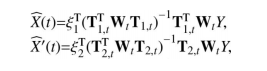
\includegraphics{images/Parameter_Estimation.png}
\caption{}
\end{figure}

where

\begin{figure}[htbp]
\centering
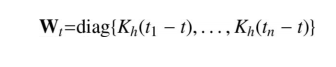
\includegraphics{images/2_stage_form_reg_W.png}
\caption{}
\end{figure}

and K(.) is a symmetric kernel function \(K_{h}\)(.) = K(./h)/h and h is
a proper bandwidth.

Currently, the implementation supports \textbf{Epanechnikov},
\textbf{Uniform} and \textbf{Triangular} kernel functions. I propose to
include more kernels such as Quartic, Triweight, Tricube, Gaussian,
Cosine, Logistic, Sigmoid function, and Silverman.

I also plan to include the advantages and the disadvantages of this
method such as :

\textbf{Advantages}

\begin{enumerate}
\def\labelenumi{\arabic{enumi}.}
\tightlist
\item
  Computational efficiency
\item
  Easing of the convergence problem
\item
  The initial values of the state variables of the differential
  equations not required
\item
  Providing good initial estimates of the unknown parameters for other
  computationally-intensive methods to further refine the estimates
  rapidly
\end{enumerate}

\textbf{Disadvantage}

\begin{enumerate}
\def\labelenumi{\arabic{enumi}.}
\tightlist
\item
  This method does not converge to the global/local minima as the
  Non-Linear regression does in the objective function is
  convex/concave.
\end{enumerate}

    \subsection{Implement support for different distance measures such as
(log-)likelihood and expectation maximization (EM)
algorithm}\label{implement-support-for-different-distance-measures-such-as-log-likelihood-and-expectation-maximization-em-algorithm}

In the present implementation the ``build\_loss\_objective'' function
only covers the Least-Square objective function and the function defined
in \href{https://github.com/JuliaML/LossFunctions.jl}{LossFunctions.jl}.
It also assumes that the errors in measurement are not correlated i.e

\begin{figure}[htbp]
\centering

\includegraphics{images/Maximum_Likelihood_no_covariance.png}
\caption{}
\end{figure}

    Then the maximum likelihood estimate of x given observations y is the
solution to the non-linear least squares problem:

~~~~~~~~~~ ~~~~~~~~~~~~~~~~~~~~~~~~~~~~~~~~~~~ \(x^{*}\) = \textbf{min}
\(||f(x)||^{2}\)

    This type of objective function can easily be constructed using
LossFunction.jl. However, there are cases when the error is correlated
such as:

    \begin{figure}[htbp]
\centering

\includegraphics{images/Maximum_Likelihood_covariance_.png}
\caption{}
\end{figure}

    then the maximum likelihood problem to be solved is:

~~~~~~~~~~ ~~~~~~~~~~~~~~~~~~~~~~~~~~~~~~~~~~~ \(x^{*}\) = \textbf{min}
f'(x)\(S^{-1}\)f(x)

    Thus, I plan to include the functionality to provide the user with the
option to state whether the errors are correlated or not and accordingly
build the cost/objective function.Also, the present implementation
assumes that the variance of the error terms is same which may always be
not the case. I will also implement an option for the \textbf{weighted
least square cost function}.

The log-likelihood function reduces to weighted least squares when the
error is normally distributed which may not be the case always. Thus,
the idea way to go about it would be to provide the option to construct
the likelihood function as the cost function. Log-likelihood should also
support different versions depending on the type of experimental noise:

\begin{enumerate}
\def\labelenumi{\arabic{enumi}.}
\tightlist
\item
  `homo' homoscedastic noise with constant variance\\
\item
  `homo\_var' homoscedastic noise with known non-constant variance
\item
  `hetero' heteroscedastic noise with variance proportional to the
  observations
\end{enumerate}

However, when we have lots of missing data or the \emph{latent variable}
for which no data has been observed, the marginal log-likelihood cost
function is multi-modal and hence very difficult to maximize. Thus, the
need for \emph{expectation maximization} algorithm.

\textbf{Expectation Maximization Algorithm}

\textbf{Assumption} - The data is drawn from the population following
the \emph{exponential family of distributions}.

The observations (\(X_{1},X_{2}\)) are drawn from the population having
probability density function \(P_{\theta}\) for some unknown \(\theta\)

\textbf{Given} - Only the observations of \(X_{1}\) is known \(x\) = (
\(x_{1},x_{2},..........\))

\textbf{Algorithm}

\begin{enumerate}
\def\labelenumi{\arabic{enumi}.}
\item
  Initialize \(\theta = \theta_{0}\)
\item
  for i in 0,1,2,\ldots{}\ldots{}.n

  \textbf{E-step} - \(Q(\theta, \theta_{i}\)) =
  \(E_{\theta_{i}}(logP_{\theta}(X1,X2)|X_{1} = x)\)

  \textbf{M-step} - \(\theta_{i+1}\) = \textbf{max}
  \(Q(\theta, \theta_{i}\))
\end{enumerate}

Repeat step 2 till the resonable convergence is obtained.

    \subsection{Implement regularization techniques such as Tikhonov
regularization, LASSO regularization and integrate with
PenaltyFunctions.jl}\label{implement-regularization-techniques-such-as-tikhonov-regularization-lasso-regularization-and-integrate-with-penaltyfunctions.jl}

Regularization aims to make the problem less complex (more regular),
i.e.~to ensure the uniqueness of the solution, to reduce the
ill-conditioning and to avoid model overfitting. These techniques are
ways to surmount ill-posedness and ill-conditioning.

For non-linear cost function, there is no general recipe for the
selection of the regularization method. The idea is to provide the users
with the options to choose from.
\href{https://github.com/JuliaML/PenaltyFunctions.jl}{PenaltyFunctions.jl}
provides two main families of penalty functions namely \textbf{Element
Penalties} and \textbf{Array Penalties} which can be used as the
regularization function.

A comprehensive list of penalty functions provided by
PenaltyFunctions.jl are:

    \textbf{Element Penalties}

\begin{longtable}[c]{@{}ll@{}}
\toprule
Penalty & value on element\tabularnewline
\midrule
\endhead
\texttt{NoPenalty()} & \texttt{g(θ)\ =\ 0}\tabularnewline
\texttt{L1Penalty()} & \texttt{g(θ)\ =\ abs(θ)}\tabularnewline
\texttt{L2Penalty()} &
\texttt{g(θ)\ =\ 0.5\ *\ θ\ \^{}\ 2}\tabularnewline
\texttt{ElasticNetPenalty(α\ =\ 0.5)} &
\texttt{g(θ)\ =\ (1\ -\ α)\ *\ abs(θ)\ +\ α\ *\ .5\ *\ θ\ \^{}\ 2}\tabularnewline
\texttt{SCADPenalty(a\ =\ 3.7,\ γ\ =\ 1.0)} &
\texttt{L1Penalty\ that\ blends\ to\ constant}\tabularnewline
\texttt{MCPPenalty(γ\ =\ 2.0)} &
\texttt{g(θ)\ =\ abs(θ)\ \textless{}\ γ\ ?\ abs(θ)\ -\ θ\ \^{}\ 2\ /\ 2γ\ :\ γ\ /\ 2}\tabularnewline
\texttt{LogPenalty(η\ =\ 1.0)} &
\texttt{g(θ)\ =\ log(1\ +\ η\ *\ abs(θ))}\tabularnewline
\bottomrule
\end{longtable}

    \textbf{Array Penalties}

\begin{longtable}[c]{@{}ll@{}}
\toprule
Penalty & value on array\tabularnewline
\midrule
\endhead
\texttt{NuclearNormPenalty()} &
\texttt{sum\ of\ singular\ values\ of\ x}\tabularnewline
\texttt{MahalanobisPenalty(C)} &
\texttt{g(x)\ =\ x\textquotesingle{}\ *\ C\textquotesingle{}\ *\ C\ *\ x}\tabularnewline
\texttt{GroupLassoPenalty()} &
\texttt{g(x)\ =\ vecnorm(x)}\tabularnewline
\bottomrule
\end{longtable}

    I propose to integrate the PenaltyFunctions.jl with DiffeEqParamEstim to
support the different penalty functions as regularization terms in the
cost function.

There are 2 other penalty type regularization techniques which should be
supported, these are:

\textbf{Tikhonov regularization}

~~~~~~~~~~ ~~~~~~~~~~~~~~~~~~~~~~~~~~~~~~~~~~~ L(\(\theta\)) =
(\(\theta - \theta^{ref})^{T} W^{T}W(\theta - \theta^{ref})\)

where W ∈ \(R^{N\theta×N\theta}\) is a diagonal scaling matrix and
\(\theta^{ref}\) ∈ \(R^{N\theta}\) is a reference parameter vector.

    \textbf{LASSO regularization}

~~~~~~~~~~ ~~~~~~~~~~~~~~~~~~~~~~~~~~~~~~~~~~~ ∑\(\theta_{i}\)
\textless{}= t

where t is the value provided by the user.

    \subsection{Provide support for deterministic and heuristic algorithms
for global optimum such as BlackBoxOptim, genetic
algorithm}\label{provide-support-for-deterministic-and-heuristic-algorithms-for-global-optimum-such-as-blackboxoptim-genetic-algorithm}

It is well-known that the cost function (5) can be highly nonlinear and
nonconvex in the model parameters. Many efficient local optimization
algorithms have been developed to find the solution of nonlinear least
squares problems, including Gauss-Newton, Levenberg-Marquardt and
trust-region methods. These local methods are especially efficient when
provided with high quality first (gradient, Jacobian) and second order
(Hessian) information via parametric sensitivities. However, in this
type of problems they will likely converge to local solutions close to
the initial guess of the parameters. Thus, there is a need to integrate
global optimization algorithm packages with DiffEqParamEstim.
\href{}{JuliaOpt} currently supports the following global optimization
algorithms:

\begin{enumerate}
\def\labelenumi{\arabic{enumi}.}
\tightlist
\item
  \href{https://github.com/robertfeldt/BlackBoxOptim.jl}{BlackBoxOptim}
  - The present cost function supports optimization using BlackBoXOptim.
  I will add an example to illustrate the users on how to use it.
\item
  \href{https://github.com/wildart/Evolutionary.jl}{Evolutionary}
  algorithms
\item
  \href{https://github.com/WestleyArgentum/GeneticAlgorithms.jl}{GeneticAlgorithms}
\item
  \href{https://github.com/phrb/StochasticSearch.jl}{StochasticSearch}
  such as Tabu Search and Simulated Annealing
\end{enumerate}

The idea is to mould the cost function (least square or likelihood)
generated during parameter estimation to be in the format accepted by
the above solvers.

\textbf{Note} - Deterministic global optimization methods can guarantee
global optimality but their computationally cost increases exponentially
with the number of estimated parameters. Alternatively, stochastic and
heuristic methods can be used as more practical alternatives, usually
obtaining adequate solutions in reasonable computation times, although
at the price of no guarantees. In such context, metaheuristics, hybrids
(i.e.~combinations) with efficient local search methods have been
particularly successful, I would also like to look at an approach to
combine the deterministic and the heuristic techniques to converge to
the exact global optimum in a reasonable time.

    \subsection{Implement Generalized Profiling Approach using Model
Relaxation method for parameter
estimation}\label{implement-generalized-profiling-approach-using-model-relaxation-method-for-parameter-estimation}

The likelihood, least squares and the two-stage methods to estimate the
parameters of the differential equations from noisy data are
computationally intensive and are often poorly suited to statistical
techniques such as inference and interval estimation. The generalized
smoothing approach is is based on the modification of data smoothing
methods along with a generalization of profiled estimation and have been
successfully deployed to find the interval estimates of the parameter.

\subsubsection{Methodology}\label{methodology}

Given the differential equation of the form:

\begin{figure}[htbp]
\centering

\includegraphics{images/smoothing_1.png}
\caption{}
\end{figure}

    The idea is to estimate the solution \(\hat{x(t)}\) as the linear
combination of the basis functions \(\phi_{i}\)(t) as:

\begin{figure}[htbp]
\centering
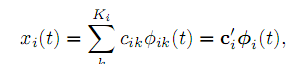
\includegraphics{images/smoothing_2.png}
\caption{}
\end{figure}

    where the number \(K_{i}\) of basis functions in vector \(\phi_{i}\) is
chosen so as to ensure enough exibility to capture the variation in xi
and its derivatives that is required to satisfy the above differential
equation.

\textbf{Note} - Although the original collocation methods used
polynomial bases, the choice of \(\phi_{i}\)(t) is taken to be spline
because of it's computational efficiency, also because it allows control
over the smoothness of the solution at specic values of t.

\textbf{The first step is to find \(c'_{i}\)} in terms of the parameter
\(\theta\) and the smoothing parameter \(\lambda\) using model fitting
and data fitting simultaneously as:

~~~~~~~~~~ ~~~~~~~~~~~~~~~~~~~~~~~~~~~~~~~~~~~
J(c\textbar{}\(\theta\),\(\sigma\),\(\lambda\)) =
\(\sum\)\(w_{i}||y_{i}-\hat{x}_{i}(t_{i})||^{2} + PEN(x|\lambda)\)

    where PEN(x\textbar{}\(\lambda\)) is given by

~~~~~~~~~~ ~~~~~~~~~~~~~~~~~~~~~~~~~~~~~~~~~~~
\(PEN(x|L_{\theta},\lambda\)) = \(\sum\lambda_{i}PEN_{i}(x)\)

and

~~~~~~~~~~ ~~~~~~~~~~~~~~~~~~~~~~~~~~~~~~~~~
\(L_{i,\theta}(x_{i}) = x_{i}^{.} - f_{i}(x,u,t|\theta)\) = 0

    Once, we have the \(c'_{i}\) the next step is to find the estimates of
the parameter \(\theta\) using data fitting as:

~~~~~~~~~~ ~~~~~~~~~~~~~~~~~~~~~~~~~~~~~~~~~~~ \textbf{Min}
\(\sum(y(t_{i})-\hat{x(t_{i})})^{2}\)

\textbf{Note} - On the computational side, this method is as fast or
faster than NLS and other approaches, and much faster than the
Bayesian-MCMC method, which has comparable estimation efficiency. Unlike
MCMC, the generalized profiling approach is relatively straightforward
to deploy to a wide range of applications.

    \subsection{Bayesian techniques for parameter estimation using
Stan.jl}\label{bayesian-techniques-for-parameter-estimation-using-stan.jl}

Stan is an open-source probabilistic programming language that performs
Bayesian inference for user-specifed models.
\href{https://github.com/goedman/Stan.jl}{Stan.jl} is the Julia
interface to the stan library.

Stan provides a built-in mechanism for specifying and solving systems of
ordinary differential equations. Stan provides two different
integrators, one tuned for solving non-stiff systems and one for stiff
systems.

\begin{itemize}
\tightlist
\item
  rk45: a fourth and fifth order Runge-Kutta method for non-stiff
  systems
\item
  bdf: a variable-step, variable-order, backward-differentiation formula
  implementation for stiff systems
\end{itemize}

\textbf{Note} - The stiff solvers are slower, but more robust.

Now, consider the ODE:

~~~~~~~~~~ ~~~~~~~~~~~~~~~~~~~~~~~~~~~~~~~~~~~ dy1 = y2 ~~~~~~~~~~
~~~~~~~~~~~~~~~~~~~~~~~~~~~~~~~~~~~ dy2 = -y1 - \(\theta\)*y2

The above ODE can be translated into DifferentialEquations format as:

    \begin{Verbatim}[commandchars=\\\{\}]
{\color{incolor}In [{\color{incolor} }]:} \PY{k}{using} \PY{n}{DifferentialEquations}
        \PY{n}{f} \PY{o}{=} \PY{p}{@}\PY{n}{ode\PYZus{}def} \PY{n}{Harmonic} \PY{k}{begin}
          \PY{n}{dy1} \PY{o}{=} \PY{n}{y2}
          \PY{n}{dy2} \PY{o}{=} \PY{o}{\PYZhy{}}\PY{n}{y1} \PY{o}{\PYZhy{}} \PY{n}{a}\PY{o}{*}\PY{n}{y2}
        \PY{k}{end} \PY{n}{a}\PY{o}{=}\PY{o}{\PYZgt{}}\PY{l+m+mf}{1.5}
        
        \PY{n}{u0} \PY{o}{=} \PY{p}{[}\PY{l+m+mf}{1.0}\PY{p}{;}\PY{l+m+mf}{1.0}\PY{p}{]}
        \PY{n}{tspan} \PY{o}{=} \PY{p}{(}\PY{l+m+mf}{0.0}\PY{p}{,}\PY{l+m+mf}{10.0}\PY{p}{)}
        \PY{n}{prob} \PY{o}{=} \PY{n}{ODEProblem}\PY{p}{(}\PY{n}{f}\PY{p}{,}\PY{n}{u0}\PY{p}{,}\PY{n}{tspan}\PY{p}{)}
\end{Verbatim}

    The above ODE is also translated into Stan program given below:

    \begin{Verbatim}[commandchars=\\\{\}]
{\color{incolor}In [{\color{incolor} }]:} \PY{n}{functions} \PY{p}{\PYZob{}}
            \PY{n}{real}\PY{p}{[}\PY{p}{]} \PY{n}{sho}\PY{p}{(}\PY{n}{real} \PY{n}{t}\PY{p}{,}
            \PY{n}{real}\PY{p}{[}\PY{p}{]} \PY{n}{y}\PY{p}{,}
            \PY{n}{real}\PY{p}{[}\PY{p}{]} \PY{n}{theta}\PY{p}{,}
            \PY{n}{real}\PY{p}{[}\PY{p}{]} \PY{n}{x\PYZus{}r}\PY{p}{,}
            \PY{n}{int}\PY{p}{[}\PY{p}{]} \PY{n}{x\PYZus{}i}\PY{p}{)} \PY{p}{\PYZob{}}
                \PY{n}{real} \PY{n}{dydt}\PY{p}{[}\PY{l+m+mi}{2}\PY{p}{]}\PY{p}{;}
                \PY{n}{dydt}\PY{p}{[}\PY{l+m+mi}{1}\PY{p}{]} \PY{o}{=} \PY{n}{y}\PY{p}{[}\PY{l+m+mi}{2}\PY{p}{]}\PY{p}{;}
                \PY{n}{dydt}\PY{p}{[}\PY{l+m+mi}{2}\PY{p}{]} \PY{o}{=} \PY{o}{\PYZhy{}}\PY{n}{y}\PY{p}{[}\PY{l+m+mi}{1}\PY{p}{]} \PY{o}{\PYZhy{}} \PY{n}{theta}\PY{p}{[}\PY{l+m+mi}{1}\PY{p}{]} \PY{o}{*} \PY{n}{y}\PY{p}{[}\PY{l+m+mi}{2}\PY{p}{]}\PY{p}{;}
            \PY{k}{return} \PY{n}{dydt}\PY{p}{;}
                \PY{p}{\PYZcb{}}
            \PY{p}{\PYZcb{}}
        \PY{n}{data} \PY{p}{\PYZob{}}
            \PY{n}{int}\PY{o}{\PYZlt{}}\PY{n}{lower}\PY{o}{=}\PY{l+m+mi}{1}\PY{o}{\PYZgt{}} \PY{n}{T}\PY{p}{;}
            \PY{n}{vector}\PY{p}{[}\PY{l+m+mi}{2}\PY{p}{]} \PY{n}{y0}\PY{p}{;}
            \PY{n}{real} \PY{n}{ts}\PY{p}{[}\PY{n}{T}\PY{p}{]}\PY{p}{;}
            \PY{n}{real} \PY{n}{theta}\PY{p}{[}\PY{l+m+mi}{1}\PY{p}{]}\PY{p}{;}
            \PY{p}{\PYZcb{}}
        \PY{n}{transformed} \PY{n}{data} \PY{p}{\PYZob{}}
            \PY{n}{real} \PY{n}{x\PYZus{}r}\PY{p}{[}\PY{l+m+mi}{0}\PY{p}{]}\PY{p}{;}
            \PY{n}{int} \PY{n}{x\PYZus{}i}\PY{p}{[}\PY{l+m+mi}{0}\PY{p}{]}\PY{p}{;}
            \PY{p}{\PYZcb{}}
        
        \PY{n}{model} \PY{p}{\PYZob{}}
            \PY{p}{\PYZcb{}}
        \PY{n}{generated} \PY{n}{quantities} \PY{p}{\PYZob{}}
            \PY{n}{vector}\PY{p}{[}\PY{l+m+mi}{2}\PY{p}{]} \PY{n}{y\PYZus{}hat}\PY{p}{[}\PY{n}{T}\PY{p}{]}\PY{p}{;}
            \PY{n}{matrix}\PY{p}{[}\PY{l+m+mi}{2}\PY{p}{,} \PY{l+m+mi}{2}\PY{p}{]} \PY{n}{A}\PY{p}{;}
            \PY{n}{A}\PY{p}{[}\PY{l+m+mi}{1}\PY{p}{,} \PY{l+m+mi}{1}\PY{p}{]} \PY{o}{=} \PY{l+m+mi}{0}\PY{p}{;}
            \PY{n}{A}\PY{p}{[}\PY{l+m+mi}{1}\PY{p}{,} \PY{l+m+mi}{2}\PY{p}{]} \PY{o}{=} \PY{l+m+mi}{1}\PY{p}{;}
            \PY{n}{A}\PY{p}{[}\PY{l+m+mi}{2}\PY{p}{,} \PY{l+m+mi}{1}\PY{p}{]} \PY{o}{=} \PY{o}{\PYZhy{}}\PY{l+m+mi}{1}\PY{p}{;}
            \PY{n}{A}\PY{p}{[}\PY{l+m+mi}{2}\PY{p}{,} \PY{l+m+mi}{2}\PY{p}{]} \PY{o}{=} \PY{o}{\PYZhy{}}\PY{n}{theta}\PY{p}{[}\PY{l+m+mi}{1}\PY{p}{]}\PY{p}{;}
            \PY{k}{for} \PY{p}{(}\PY{n}{t} \PY{k}{in} \PY{l+m+mi}{1}\PY{p}{:}\PY{n}{T}\PY{p}{)}
            \PY{n}{y\PYZus{}hat}\PY{p}{[}\PY{n}{t}\PY{p}{]} \PY{o}{=} \PY{n}{matrix\PYZus{}exp}\PY{p}{(}\PY{p}{(}\PY{n}{t} \PY{o}{\PYZhy{}} \PY{l+m+mi}{1}\PY{p}{)} \PY{o}{*} \PY{n}{A}\PY{p}{)} \PY{o}{*} \PY{n}{y0}\PY{p}{;}
            \PY{o}{/}\PY{o}{/} \PY{n}{add} \PY{n}{measurement} \PY{n+nb}{error}
            \PY{k}{for} \PY{p}{(}\PY{n}{t} \PY{k}{in} \PY{l+m+mi}{1}\PY{p}{:}\PY{n}{T}\PY{p}{)} \PY{p}{\PYZob{}}
                \PY{n}{y\PYZus{}hat}\PY{p}{[}\PY{n}{t}\PY{p}{,} \PY{l+m+mi}{1}\PY{p}{]} \PY{o}{=} \PY{n}{y\PYZus{}hat}\PY{p}{[}\PY{n}{t}\PY{p}{,} \PY{l+m+mi}{1}\PY{p}{]} \PY{o}{+} \PY{n}{normal\PYZus{}rng}\PY{p}{(}\PY{l+m+mi}{0}\PY{p}{,} \PY{l+m+mf}{0.1}\PY{p}{)}\PY{p}{;}
                \PY{n}{y\PYZus{}hat}\PY{p}{[}\PY{n}{t}\PY{p}{,} \PY{l+m+mi}{2}\PY{p}{]} \PY{o}{=} \PY{n}{y\PYZus{}hat}\PY{p}{[}\PY{n}{t}\PY{p}{,} \PY{l+m+mi}{2}\PY{p}{]} \PY{o}{+} \PY{n}{normal\PYZus{}rng}\PY{p}{(}\PY{l+m+mi}{0}\PY{p}{,} \PY{l+m+mf}{0.1}\PY{p}{)}\PY{p}{;}
                \PY{p}{\PYZcb{}}
            \PY{p}{\PYZcb{}}
\end{Verbatim}

    \textbf{Our objective is to translate the ODE described in
DifferentialEquations.jl using ParameterizedFunctions.jl into the
corresponding Stan above and use Stan.jl to find the Bayesian estimates
of the parameters.}

Fortunately, ParametrizedFunctions.jl already provides us the option to
extract the information the ODE model such as:

    \begin{Verbatim}[commandchars=\\\{\}]
{\color{incolor}In [{\color{incolor}7}]:} \PY{n}{println}\PY{p}{(}\PY{n}{f}\PY{o}{.}\PY{n}{origex}\PY{p}{)}
\end{Verbatim}

    \begin{Verbatim}[commandchars=\\\{\}]
begin  \# In[6], line 3:
    dy1 = y2 \# In[6], line 4:
    dy2 = -y1 - a * y2
end

    \end{Verbatim}

    \begin{Verbatim}[commandchars=\\\{\}]
{\color{incolor}In [{\color{incolor}8}]:} \PY{n}{println}\PY{p}{(}\PY{n}{f}\PY{o}{.}\PY{n}{params}\PY{p}{)} \PY{c}{\PYZsh{} prints the parameter of the differential equation}
\end{Verbatim}

    \begin{Verbatim}[commandchars=\\\{\}]
Symbol[:a]
Expr[quote 
    du[1] = 1 * u[2]
    du[2] = -(u[1]) - a * u[2]
    nothing
end]

    \end{Verbatim}

    To summarize the above process in 3 steps: 1. Express the ODE model in
Julia using \texttt{ParametrizedFunctions.jl}. 2. Convert the
ParametrizedFunctions ODE model to Stan model using the functionalities
provided by ParametrizedFunctions 3. Use Stan.jl to generate posterior
distribution of parameters and return it to the user

    \section{About Me}\label{about-me}

\subsection{Personal Background}\label{personal-background}

I am a final year graduate student pursuing an Integrated Master of
Science(MS) degree in Mathematics and Computing Sciences with
specialization in Optimization at IIT Kharagpur, India. I am proficient
in C, C++, Python, and Julia.

\subsection{Previous Relevant
Experience}\label{previous-relevant-experience}

I am a former Google Summer of the Code student with the Julia Language
where I worked on the project titled \textbf{Support for complex numbers
within Convex.jl}. As a result of our work, we became the first
open-source DCP package to support optimization with complex-variables.
I have also worked on different projects related to optimization and
machine learning. Please find all my projects
\href{https://drive.google.com/drive/folders/0B2oOdWdSJWa1RWRsQWdCZ25LUXc}{here}.
I have taken courses on differential equations such as Partial
Differential Equations, Numerical solution of ODE and PDE and Advanced
NUmnerical Techniques(Theory and Lab) where I have written MATLAB/C
\href{https://github.com/Ayush-iitkgp/Numerical-Solution-of-ODE-and-PDE}{code}
for different numerical techniques used in solving ODEs and PDEs.

\subsection{Relevant Courses}\label{relevant-courses}

\begin{itemize}
\tightlist
\item
  Partial Differential Equations
\item
  Numerical solution of ODE and PDE
\item
  Advanced Numerical Techniques
\item
  Stochastic Processes
\item
  Non-Linear Programming
\item
  Convex Optimization
\item
  Probability \& Statistics, Regression, Generalized Linear Models
\item
  Linear Algebra, Programming and Data Structures, Object Oriented
  System Design
\end{itemize}

\subsection{Answers of listed
questions}\label{answers-of-listed-questions}

\texttt{1.\ What\ do\ you\ want\ to\ have\ completed\ by\ the\ end\ of\ the\ program?}

By the end of the program, I want to support different optimization and
bayesian techniques used to estimate the parameters of the differential
equations given the experimental data. Presently, DiffEqParamEstim only
supports Non-Linear Regression technique to estimate the parameters. I
aim to implement numerous techniques such as two-stage method, model
relaxation technique, regularization, log-likelihood estimation,
meta-heuristic techniques for global optimum and bayesian techniques
using Stan.jl.

\texttt{2.\ Who’s\ interested\ in\ the\ work,\ and\ how\ will\ it\ benefit\ them?}

The problem of parameter estimation has extensive use in the following
fields: 1. HIV-AIDS viral dynamics 2. Systems biology 3. Drug dosage
estimation

\texttt{3.\ What\ are\ the\ potential\ hurdles\ you\ might\ encounter,\ and\ how\ can\ you\ resolve\ them?}

In order to link Stan with DiffEqParamEstim, I will have to understand
how Stan works. I will also need to go through the theory of Markov
Chain Monte Carlo and Hamiltonian Monte Carlo to write in-situ Bayesian
estimator for parameters of the differential equations. Lastly, I would
need to understand the theory behind the stochastic differential
equations to write an implementation to find it's parameters.

\texttt{4.\ How\ will\ you\ prioritize\ different\ aspects\ of\ the\ project\ like\ features,\ API\ usability,\ documentation,\ and\ robustness?}

Please refer to the ``Timeline'' section where I have described in
details about my plans to tackle different aspects of the project.

\texttt{5.\ Does\ your\ project\ have\ any\ milestones\ that\ you\ can\ target\ throughout\ the\ period?}

Yes, before JuliaCon 2017, I would have implemented the various
optimization and regularization algorithms to estimate the parameters
and would be ready for testing for the Julia community.

\texttt{6.\ Are\ there\ any\ stretch\ goals\ you\ can\ make\ if\ the\ main\ project\ goes\ smoothly?}

Yes, I would try to implement native Julia computational engine for
Bayesian estimation using tools like Mamba.jl or Klara.jl and the
inverse problem for Stochastic Differential Equations based on the paper
\href{http://journals.aps.org/prx/abstract/10.1103/PhysRevX.5.031036}{Control
of Stochastic and Induced Switching in Biophysical Networks}.

\texttt{7.\ What\ other\ time\ commitments,\ such\ as\ summer\ courses,\ other\ jobs,\ planned\ vacations,\ etc.,\ will\ you\ have\ over\ the\ summer?}

I expect to work full time on the project that is 30 or more hours a
week.

\subsection{Contribution to Open-Source
Projects}\label{contribution-to-open-source-projects}

\begin{itemize}
\item
  \href{https://github.com/JuliaOpt/Convex.jl/pulls?q=is:pr+author:Ayush-iitkgp+is:closed}{List}
  of all Pull Requests to Convex.jl
\item
  Added two-stage method
  \href{https://github.com/JuliaDiffEq/DiffEqParamEstim.jl/pull/6}{\#6}
\item
  \href{https://github.com/JuliaDiffEq/DiffEqDocs.jl/pulls?q=is:pr+author:Ayush-iitkgp+is:closed}{Improved
  DiffEqDocs}.
\item
  Implemented
  \href{https://github.com/Ayush-iitkgp/Heuristic-Optimization}{Genetic
  Algorithm}for heuristic optimization
\item
  Elaborated installation instruction for SCIP.jl
  \href{https://github.com/SCIP-Interfaces/SCIP.jl/pull/35}{\#35}
\end{itemize}

\subsection{Experience with Julia}\label{experience-with-julia}

I have been using Julia for last one year. In terms of functionality, I
like Julia because of its \textbf{multiple dispatch} feature as it lets
me overload operators with a lot of ease than other programming
languages.

But the most astonishing feature of Julia is that it is empowering. In
other high-level languages, the users can not be developers because
developing new packages in those languages require the users to know the
intricacies of low-level language whereas, in Julia, users can develop
packages for their needs in Julia itself without compromising with the
speed.

    \section{Timeline (tentative)}\label{timeline-tentative}

    \subsubsection{Community Bonding period (May 5 - 30,
2017)}\label{community-bonding-period-may-5---30-2017}

My summer vacation will start from 6th of May. During this period, I
would want to get myself more familiarized with the other similar
projects in languages like MATLAB, python. The idea to take an
inspiration from the similar mature projects so that we understand the
potential user's requirements, have an idea of the structure of the API
we provide to the users so that it is very easy to switch to out
implementation once we are ready to get released.

I would also like to use this time to understand the intricacies of
Stochastic Differential Equation Models and probabilistic programming
language Stan to help me figure out how to provide a support for it in
DiffEqParamEstim.

    \subsubsection{Week 1}\label{week-1}

\textbf{Goal:} \emph{Implement support for more Kernels for two-stage
method}

I plan to implement the different techniques and algorithms described in
the ``Execution'' section on weekly basis. We can merge the code in the
main project after each method is implemented. The end outcome of this
week would be that the users would be able to provide an option for more
kernel functions while using the two-stage method.

    \subsubsection{Week 2, 3 and 4}\label{week-2-3-and-4}

\textbf{Goal:} \emph{Implement support for different distance measures
such as (log-)likelihood and expectation }

In this week, I plan to implement the support for log-likelihood cost
function which is expected to take 1 week at maximum. Week 3 and 4 would
be utilized to implement the second part which is \textbf{Expectation
maximization algorithm}.

    \subsubsection{Week 5 and 6}\label{week-5-and-6}

\textbf{Goal:} \emph{Integrate with PenaltyFunctions.jl and implement
Tikhonov and Lasso regularization}

These 2 weeks would be required to implement regularization techniques
such as Tikhonov regularization, LASSO regularization and integrate
DiffEqParamEstim with PenaltyFunctions.

    \subsubsection{Week 7 and 8}\label{week-7-and-8}

\textbf{Goal:} \emph{Documentation for JuliaCon and attending JuliaCon}

By this time, we would have a general set-up for finding the parameters
of the differential equations using optimization techniques. If selected
for JuliaCon 2017, I would like to take this time to write an easy to
understand documentation of the methods implemented so far and travel to
Berkeley to present my work.

    \subsubsection{Week 8}\label{week-8}

\textbf{Goal:} \emph{Provide support for deterministic and heuristic
algorithms for global optimum such as BlackBoxOptim, genetic algorithm }

During this week, I plan to add the support for the 4 packages mentioned
in my proposal to find the global optimum for the parameter estimation.

    \subsubsection{Week 9 and 10}\label{week-9-and-10}

\textbf{Goal:} \emph{Implement Generalized Profiling Approach using
Model Relaxation method for parameter estimation}

    \subsubsection{Week 11 and 12}\label{week-11-and-12}

\textbf{Goal:} \emph{Link with Stan.jl to estimate the parameters using
Bayesian inference}

    \subsubsection{End-Term evaluation}\label{end-term-evaluation}

\textbf{Goal:} \emph{Working to implement the strech goals}

Buffer period for any lagging work. I also aim to work towards
implementing the stretch goals such as to implementing support for
parameter estimation for stochastic differential equations and write
native Julia bayesian computational engine using Mamba.jl and Klara.jl.

    \section{References}\label{references}

{[}1{]}.
\href{https://www.ncbi.nlm.nih.gov/pmc/articles/PMC2631937/}{Parameter
Estimation for Differential Equation Models Using a Framework of
Measurement Error in Regression Models}

{[}2{]}. Parameter estimation: the build\_loss\_objective
\href{https://github.com/JuliaDiffEq/DiffEqParamEstim.jl/issues/5}{\#5}

{[}3{]}.
\href{https://github.com/JuliaML/PenaltyFunctions.jl}{PenaltyFunctions.jl}

{[}4{]}.
\href{http://bmcsystbiol.biomedcentral.com/articles/10.1186/s12918-015-0219-2}{Robust
and efficient parameter estimation in dynamic models of biological
systems}

{[}5{]}.
\href{http://faculty.bscb.cornell.edu/~hooker/ODE_Estimation.pdf}{Parameter
Estimation for Differential Equations: A Generalized Smoothing Approach}

{[}6{]}.
\href{http://www.stat.columbia.edu/~gelman/research/published/stan_jebs_2.pdf}{Stan:
A probabilistic programming language for Bayesian inference and
optimization}

{[}7{]}. Linking with Stan project
\href{https://github.com/JuliaDiffEq/DifferentialEquations.jl/issues/135}{\#135}


    % Add a bibliography block to the postdoc
    
    
    
    \end{document}
